\documentclass[12pt,a4paper,pdflatex]{disser}
\usepackage[russian]{babel}
%\usepackage[utf-8]{inputenc}
%\usepackage{amsmath,amssymb}
%\usepackage{longtable}
\usepackage{parskip}
\usepackage{caption}
\usepackage{textcomp}
\usepackage{gensymb}
\usepackage[dvips]{graphicx}
%\usepackage{wrapfig}
%\usepackage{amssymb}*
%\usepackage{color}
%\usepackage{ulem}
\usepackage{setspace}
\usepackage{hyperref}

\oddsidemargin=-0.5 cm
\evensidemargin=-0.5 cm
\textwidth=170 mm
\textheight=260 mm
\topmargin=0 cm
\voffset= -2cm
\pagenumbering{true}
%\newlength{\varheight}
%\setlength{\varheight}{3.1cm}
\setlength{\parindent}{0cm}
%\newcommand{\taskname}[name]{\begin{center} \bf{\Large{name}} \end{center}}
\spacing{1.1}
\parskip=2mm
\captionsetup[figure]{labelformat=empty}
\clubpenalty=10000
\widowpenalty=10000

\begin{document}

\begin{wrapfigure}{r}{160pt}
\vspace{-1mm}
\begin{center}
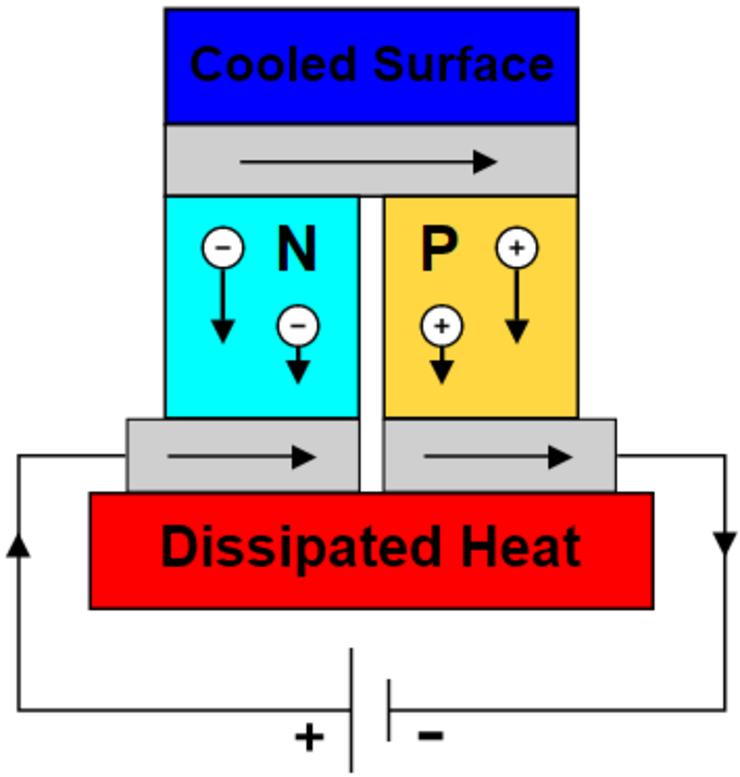
\includegraphics[scale=0.5]{peltier.pdf}
\end{center}
\caption{To solution 1}
\vspace{-10mm}
\end{wrapfigure}
1. The idea is to apply voltage to the free ends of the leads and heat them. Then the connected ends will be cooled (see picture\footnote{Source \href{https://upload.wikimedia.org/wikipedia/commons/3/3b/Thermoelectric_Cooler_Diagram.svg}{here}}).

2. The Hall voltage is defined by the formula
$$
  V=\frac{BI}{ned},
$$
which implies
$$
  n=\frac{BI}{eVd}=7.72\cdot 10^{28} \text{ m}^{-3}.
$$

3. Usually phosphorus is used in agriculture. As the $^{31}$P isotope is stable, then the radioisotope is $^{32}$P.

4. Relativistic effects are ignored in the solution. The number of protons which cross a unit area near the Earth's orbit is
$$
  \frac{dN}{dS}=nv.
$$
Each proton can deliver a maximum momentum of $p_0=2mv$. Let's consider that in average a proton delivers a momentum $p=mv$. Then the pressure of the solar wind is
$$
  f=p\frac{dN}{dS}=nmv^2=4.2\cdot 10^{-9} \text{ Pa}.
$$

5. Star formation and dynamics problems are frequently chosen for the IPhO, last ones are \href{http://ipho.phy.ntnu.edu.tw/problems-and-solutions/2009/IPhO_2009_Theo_Problem 3.pdf}{2009.3} and \href{http://ipho.phy.ntnu.edu.tw/problems-and-solutions/2012/2012-08-09 IPhO2012_Theoretical_problems.pdf}{2012.3}. The collapse is stopped by the pressure of the hot electron gas. When the stellar hydrogen is over, then the collapse may continue (in case of a sufficiently big star mass), as the temperature increases.

6. This problem was met in a variety of papers, for example, in ``Problems in physics''\footnote{Link \href{http://zfmsh.nsu.ru/zfmsh/html/biblio/articles/phys/zadach.pdf}{here}}, and in the IPhO as the problem \href{http://ipho.phy.ntnu.edu.tw/problems-and-solutions/1987/18th_IPhO_1987.pdf}{1987.3}. The dispersion relation is
$$
  \omega(\lambda)=\frac{2}{\sqrt{LC}}\sin\frac{\pi l}{\lambda},
$$
the cut-off happens when $\omega=2/\sqrt{LC}$.

\end{document} 